\documentclass[11pt,letterpaper]{article}

% \usepackage{epstopdf}% To incorporate .eps illustrations using PDFLaTeX, etc.
% \usepackage[caption=false]{subfig}% Support for small, `sub' figures and tables
%\usepackage[nolists,tablesfirst]{endfloat}% To `separate' figures and tables from text if required
%\usepackage[doublespacing]{setspace}% To produce a `double spaced' document if required
%\setlength\parindent{24pt}% To increase paragraph indentation when line spacing is doubled

% \usepackage[longnamesfirst,sort]{natbib}% Citation support using natbib.sty
% \bibpunct[, ]{(}{)}{;}{a}{,}{,}% Citation support using natbib.sty
% \renewcommand\bibfont{\fontsize{10}{12}\selectfont}% To set the list of references in 10 point font using natbib.sty

\usepackage[natbibapa,nodoi]{apacite}% Citation support using apacite.sty. Commands using natbib.sty MUST be deactivated first!
\setlength\bibhang{12pt}% To set the indentation in the list of references using apacite.sty. Commands using natbib.sty MUST be deactivated first!
\renewcommand\bibliographytypesize{\fontsize{10}{12}\selectfont}% To set the list of references in 10 point font using apacite.sty. Commands using natbib.sty MUST be deactivated first!

% \theoremstyle{plain}% Theorem-like structures provided by amsthm.sty
% \newtheorem{theorem}{Theorem}[section]
% \newtheorem{lemma}[theorem]{Lemma}
% \newtheorem{corollary}[theorem]{Corollary}
% \newtheorem{proposition}[theorem]{Proposition}

% \theoremstyle{definition}
% \newtheorem{definition}[theorem]{Definition}
% \newtheorem{example}[theorem]{Example}

% \theoremstyle{remark}
% \newtheorem{remark}{Remark}
% \newtheorem{notation}{Notation}

\usepackage[table,x11names,svgnames,dvipsnames]{xcolor}
\usepackage[export]{adjustbox}
% \usepackage{algorithm}
% \usepackage[noend]{algpseudocode}
\usepackage{amsmath,amssymb,amsfonts}
\usepackage[USenglish]{babel}
\usepackage{bigints}
\usepackage{bm}
\usepackage{booktabs}
\usepackage{cancel}
\usepackage[tableposition=above, font=normalsize]{caption}
% \usepackage{centernot}
% \usepackage{comment}
\usepackage{empheq}
\newcommand*\widefbox[1]{\fbox{\hspace{2em}#1\hspace{2em}}}
\usepackage{enumitem}
\usepackage{epsfig}
\usepackage{epstopdf}
% \epstopdfsetup{outdir=./figures//}
% \usepackage[letterpaper, top=1.0in, bottom=1.0in, left=1.0in, right=1.0in]{geometry}
\RequirePackage[OT1]{fontenc}
% \usepackage{fontspec}
\usepackage{graphics}
\usepackage{graphicx}
\graphicspath{{../figures/}}
% \usepackage{ifpdf}
% \usepackage{lastpage}
% \usepackage{leftidx}
\usepackage{lineno}
\usepackage{lipsum}
% \usepackage{mathrsfs}
\usepackage{mathtools}
\usepackage{multicol}
\usepackage{multirow}
\usepackage{nicefrac}
% \usepackage{nicematrix}
% \usepackage{pgfplots}
\usepackage{pifont}
% \usepackage{ragged2e}
% \usepackage{rotating}
% \usepackage{stmaryrd}
\usepackage{siunitx}
\usepackage{soul}
\usepackage[caption=false]{subfig}
\usepackage{tabularx}
\usepackage{threeparttable}
\usepackage{tikz}
% \usepackage{tkz-euclide}
% \usepackage{ctable}
% \usetikzlibrary{matrix, arrows}
\usetikzlibrary{shapes.geometric, arrows, decorations.markings, shapes.arrows}

\newcommand{\minitab}[2][l]{\begin{tabular}{#1}#2\end{tabular}}

%%%%%%% TODO NOTES 
\usepackage{todonotes}
\setlength{\marginparwidth}{1.3cm}
\setlength{\marginparsep}{0cm}
\newcommand{\ctodo}[1]{\todo[size=\tiny]{#1}}
\newcommand{\nnparam}{\theta}
\newcommand{\pinn}{\pi_{\nnparams}}

\usepackage{ulem}
\usepackage{wrapfig}

\tikzstyle{startstop} = [rectangle, rounded corners, minimum width=1cm, minimum
height = 0.5cm, text centered, draw=black, fill=red!30]
\tikzstyle{io} = [trapezium, trapezium left angle=70, trapezium right angle=110,
minimum height=1cm, text width=3cm, text centered, draw=black, fill=blue!30]
\tikzstyle{process} = [rectangle, minimum width=2cm, minimum height=0.8cm, text
centered, text width=2cm, draw=black, fill=orange!30]
\tikzstyle{decision} = [diamond, aspect=1.25, minimum width=2cm, minimum height=0.5cm, 
text centered, text width=3cm, draw=black, fill=green!30]
\tikzstyle{arrow} = [thick, ->, >=stealth]




\makeatletter
\newcommand{\rmnum}[1]{\romannumeral #1}
\newcommand{\Rmnum}[1]{\expandafter\@slowromancap\romannumeral #1@}
\makeatother

\DeclarePairedDelimiter\ceil{\lceil}{\rceil}
\DeclarePairedDelimiter\floor{\lfloor}{\rfloor}

\newcommand{\bmat}[1]{\begin{bmatrix}#1\end{bmatrix}}
\newcommand{\pmat}[1]{\begin{pmatrix}#1\end{pmatrix}}
\newcommand{\ubar}[1]{\text{\b{$#1$}}}
\newcommand{\norm}[2]{\|{#1}\|_{{}_{#2}}}
\newcommand{\abs}[1]{\left|{#1}\right|}
\newcommand{\mbf}[1]{\mathbf{#1}}
\newcommand{\mc}[1]{\mathcal{#1}}
\newcommand{\dd}{\operatorname{d}\!}
\newcommand{\muc}[2]{\multicolumn{#1}{c}{#2}}
\newcommand*\Eval[3]{\left.#1\right\rvert_{#2}^{#3}}
\newcommand{\inner}[1]{\left\langle#1\right\rangle}
\newcommand{\pd}[2]{\frac{\partial #1}{\partial #2}}
\newcommand{\pdd}[2]{\frac{\partial^2 #1}{\partial #2^2}}
\newcommand{\el}[2]{\frac{\dd}{\dd t}\pd{\mc{L}}{\dot{#1}} - \pd{\mc{L}}{#1} = #2}
\newcommand{\elk}[2]{\frac{\dd}{\dd t}\pd{\mc{L}}{\dot{#1}_k} - \pd{\mc{L}}{#1_k} = #2_k}
\newcommand{\vectornorm}[1]{\left|\left|#1\right|\right|}
\newcommand{\dom}[1]{\textrm{dom}\;#1}
\newcommand{\bx}{{\bf x}}
\newcommand{\bu}{{\bf u}}
\newcommand{\cmark}{\ding{51}}%
\newcommand{\xmark}{\ding{55}}%
\newcommand*{\vertbar}{\rule[-1ex]{0.5pt}{2.5ex}}
\newcommand*{\horzbar}{\rule[.5ex]{2.5ex}{0.5pt}}

\newcommand{\idapbc}{\textsc{IdaPbc}}
\newcommand{\electric}{{\textcolor{blue}{\hspace{-0.5mm}$\bm{E}$\;}}}
\newcommand{\magnetic}{{\textcolor{red}{\hspace{-0.5mm}$\bm{B}$\;}}}

% \theoremstyle{plain}
% \newtheorem{thm}{Theorem}[section]
\newtheorem{thm}{Theorem}
% \makeatletter
% \@addtoreset{thm}{section}
% \makeatother
% \newtheorem{cor}[thm]{Corollary}
\newtheorem{lem}{Lemma}
% \newtheorem{claim}[thm]{Claim}
% \newtheorem{axiom}[thm]{Axiom}
% \newtheorem{conj}[thm]{Conjecture}
% \newtheorem{fact}[thm]{Fact}
% \newtheorem{hypo}[thm]{Hypothesis}
% \newtheorem{assum}[thm]{Assumption}
\newtheorem{prop}{Proposition}
% \newtheorem{crit}[thm]{Criterion}
% \theoremstyle{definition}
\newtheorem{defn}[thm]{Definition}
% \newtheorem{exmp}[thm]{Example}
\newtheorem{rem}{Remark}
% \newtheorem{prin}[thm]{Principle}

\DeclareMathOperator{\Tr}{tr}
\newcommand\xdownarrow[1][2ex]{%
   \mathrel{\rotatebox{90}{$\xleftarrow{\rule{#1}{0pt}}$}}
}
\DeclareMathOperator{\End}{End}
\DeclareMathOperator{\Hom}{Hom}
\DeclareMathOperator{\id}{id}
\DeclareMathOperator{\vers}{vers}
\DeclareMathOperator{\trans}{Trans}
\DeclareMathOperator{\rot}{Rot}
\DeclareMathOperator{\rank}{rank}
\DeclareMathOperator{\sinc}{sinc}

\usepackage{hyperref}
\hypersetup{
    unicode=false,          % non-Latin characters in Acrobat’s bookmarks
    pdftoolbar=true,        % show Acrobat’s toolbar?
    pdfmenubar=true,        % show Acrobat’s menu?
    pdffitwindow=false,     % window fit to page when opened
    pdfstartview={FitH},    % fits the width of the page to the window
    pdftitle={Mischievous Sibling's Grid World},    % title
    pdfauthor={Aykut C. Satici}, % author
    % pdfsubject={Subject},   % subject of the document
    % pdfcreator={Creator},   % creator of the document
    % pdfproducer={Producer}, % producer of the document
    % pdfkeywords={keyword1, key2, key3}, % list of keywords
    pdfnewwindow=true,      % links in new PDF window
    colorlinks=true,       % false: boxed links; true: colored links
    linkcolor=blue!30!green,          % color of internal links (change box color with linkbordercolor)
    linkbordercolor=orange,
    citecolor=blue,        % color of links to bibliography
    citebordercolor=green,
    filecolor=magenta,      % color of file links
    urlcolor=cyan,           % color of external links
    urlbordercolor=blue,
}


\begin{document}

% \articletype{}% Specify the article type or omit as appropriate

% \title{\.{I}lgin\c{c} Bir Olas{\i}l{\i}k Sorusu}
\section*{
    \begin{center}
        An Interesting Probability Question
    \end{center}
}

\begin{center}
    G\"{o}khan At{\i}n\c{c}\textsuperscript{} and Aykut C. Sat{\i}c{\i}\textsuperscript{} \\[0ex]
    % 1 Temmuz 2021
\end{center}


  
\vspace{-1mm}
\section{Problem Statement}
%
% \begin{wrapfigure}{r}{0.4\textwidth} %this figure will be at the right
%     \vspace{-5mm}
%     \centering
%     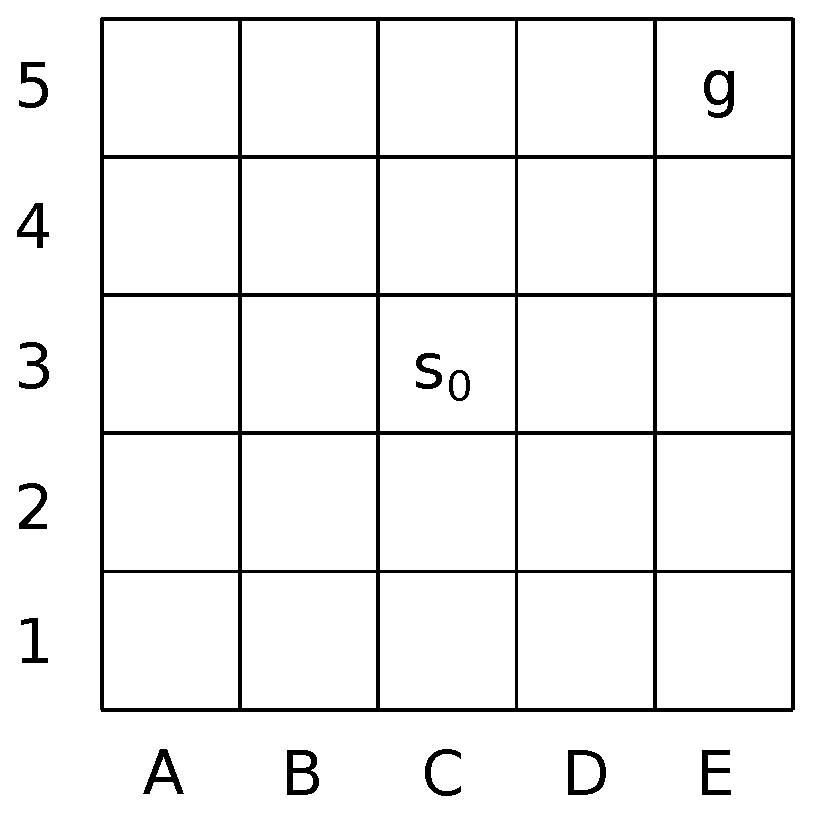
\includegraphics[width=0.25\textwidth]{./figures/drawing.eps}
%     \caption{Problemin \c{s}emati\u{g}i}
%     \label{fig:schematic}
%     \vspace{-5mm}
% \end{wrapfigure}
%
\begin{minipage}{0.5\textwidth}
    Consider the blue rectangle that shares its bottom left corner with that of
    the triangle $\triangle ABC$ as seen in the figure to the right. The length
    of the line segment between points $B$ and the top left corner of the
    rectangle is $4$ units while the length of the line segment between the
    bottom right corner of the rectangle and point $C$ is $3$  units.
\end{minipage}
\begin{minipage}{0.5\textwidth}
\begin{tikzpicture}[scale=0.85]
\tkzInit[xmax=8, ymax=8/3]
% \tkzDefPoint(0,0){B}
\tkzDefPoint(0,0){A}
\tkzDefPoint(8,0){C}
\tkzDrawTriangle[two angles = 90 and 18.43494882292201](A,C)
\tkzGetPoint{B}
\tkzLabelPoints[below left](A)
\tkzLabelPoints[below right](C)
\tkzLabelPoints[above left](B)

\tkzDefPoint(0,1){D}
\tkzDefPoint(5,0){E}
\tkzDefPoint(5,1){F}
\tkzDrawPolygon[fill=black!50!blue!20!, opacity=0.75](A,D,F,E)
% \tkzLabelPoints[below](E)
% \tkzLabelPoints[left](D)

\tkzMarkRightAngles(C,A,tkzPointResult)
\tkzDrawPoints(A,B,C)

\tkzDefPoint(5,-0.1){E1}
\tkzDefPoint(5,-0.3){E2}
\tkzDrawSegment[color=black](E1,E2)
\tkzDefPoint(8,-0.1){C1}
\tkzDefPoint(8,-0.3){C2}
\tkzDrawSegment[color=black](C1,C2)
\tkzDefMidPoint(E1,E2) \tkzGetPoint{E12mid}
\tkzDefMidPoint(C1,C2) \tkzGetPoint{C12mid}
\tkzDrawSegment[color=black](E12mid,C12mid)

\tkzDefPoint(-0.1,8/3){B1}
\tkzDefPoint(-0.3,8/3){B2}
\tkzDrawSegment[color=black](B1,B2)
\tkzDefPoint(-0.1,1){D1}
\tkzDefPoint(-0.3,1){D2}
\tkzDrawSegment[color=black](D1,D2)
\tkzDefMidPoint(B1,B2) \tkzGetPoint{B12mid}
\tkzDefMidPoint(D1,D2) \tkzGetPoint{D12mid}
\tkzDrawSegment[color=black](B12mid,D12mid)

\tkzLabelSegment[left, font=\footnotesize](B12mid,D12mid){4}
\tkzLabelSegment[below, font=\footnotesize](E12mid,C12mid){3}

\end{tikzpicture}
\end{minipage}

\begin{enumerate}
    \setlength\itemsep{0em}
    \item Find the area of the rectangle.
    \item What is the minimum area of the triangle $\triangle ABC$?
\end{enumerate}
\section{Problem Solution}
\label{sec:solution}

Shown in Figure~\ref{fig:unfolded}, we show the regular pyramid of
Figure~\ref{fig:problem} unfolded in a particular manner.

\begin{figure}[h]
  \centering
  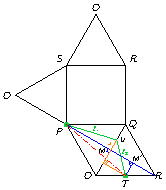
\includegraphics[trim={0 0 0
  0cm},clip,width=0.5\textwidth]{./figures/pyramid-unfolded.pdf}
  \vspace{-8mm}
  \caption{The regular pyramid unfolded.}
  \label{fig:unfolded}
\end{figure}



\bibliographystyle{apacite}
\bibliography{bib/main}

\end{document}
